\begin{notechapter}
\chapter{Classic CNN Architectures}\label{ch:cnn-architectures}
\chaptersubtitle{From LeNet to ResNet: the design ideas that made deep vision work}

\begin{chapterintro}
The architectures that won the ImageNet competition between 2012 and 2015 each
introduced one idea that is still in use: depth with small kernels, cheap $1\times1$
bottlenecks, and residual connections. This chapter goes through them with their numbers,
explains each idea quantitatively, and ends with the efficient networks that followed. You
will learn
\begin{itemize}[nosep]
  \item the structure of LeNet, AlexNet, VGG, GoogLeNet and ResNet, and their parameter
        counts;
  \item why stacks of $3\times3$ kernels beat large kernels;
  \item how $1\times1$ bottlenecks cut the cost of an Inception module by an order of magnitude;
  \item what a residual connection does to the forward signal and to the gradient, precisely;
  \item the ideas behind MobileNet and EfficientNet.
\end{itemize}
\prerequisites{\cref{ch:convolutional-layers}; vanishing gradients
(\cref{activation-functions:sec:vanishing}); batch normalization (\cref{ch:normalization}).}
\end{chapterintro}

\section{The setting: ImageNet}\label{cnn-architectures:sec:imagenet}

The ImageNet Large Scale Visual Recognition Challenge (ILSVRC; Russakovsky et al., IJCV,
2015) asked for the classification of images into $1000$ classes, with $1.28$ million training images.
Performance is reported as the \emph{top-5 error}: the fraction of test images whose true class is
not among the five highest-scoring classes. In 2011 the best entry, based on hand-designed
features, had a top-5 error of about $26\%$. Four years later, CNNs were below $4\%$. All the networks
below take $224\times224$ RGB inputs (AlexNet $227\times227$), standardized per channel
(\cref{transfer-learning:sec:preprocessing}).

\section{LeNet and AlexNet}\label{cnn-architectures:sec:alexnet}

\paragraph{LeNet-5} (LeCun, Bottou, Bengio and Haffner, \emph{Gradient-Based Learning
Applied to Document Recognition}, Proceedings of the IEEE, 1998) recognized $32\times32$
handwritten digits with two convolutional layers ($5\times5$ kernels, $6$ then $16$ channels), each followed
by subsampling, and three fully connected layers: about $60\,000$ parameters. Its pattern,
convolutions and pooling that shrink the image while increasing the channels, then fully
connected layers, is the template of all classic CNNs.

\paragraph{AlexNet} (Krizhevsky, Sutskever and Hinton, \emph{ImageNet Classification with
Deep Convolutional Neural Networks}, NIPS, 2012) won ILSVRC 2012 with a top-5 error of
$15.3\%$, against $26.2\%$ for the second entry. It has five convolutional layers (the first with $11\times11$
kernels and stride $4$) and three fully connected layers, about $61$ million parameters, of which
$58$ million are in the fully connected layers. Its ingredients, all now standard, were: ReLU
activations (\cref{ch:activation-functions}), dropout in the fully connected layers
(\cref{ch:dropout}), data augmentation (random crops and flips), and training on two
GPUs.

\section{VGG: depth with small kernels}\label{cnn-architectures:sec:vgg}

VGG (Simonyan and Zisserman, \emph{Very Deep Convolutional Networks for Large-Scale Image
Recognition}, ICLR, 2015) uses only $3\times3$ convolutions with stride $1$ and padding $1$, and $2\times2$ max pooling.
VGG-16 has $13$ convolutional layers in five blocks, with $64, 128, 256, 512, 512$ channels, the
spatial size halved after each block, then three fully connected layers
(\cref{cnn-architectures:fig:vgg}).

\begin{figure}[ht]
\centering
\begin{tikzpicture}[x=1cm, y=1cm]
  \def\nnbaseline{-1.8}
  \nnbox{in}{0}{0.08}{3.4}{3.4}{gray}{$3$\\$224^2$}
  \nnbox{b1}{1.9}{0.35}{3.4}{3.4}{bookaccent}{$2\times$conv\\$64$, $224^2$}
  \nnbox{b2}{4.1}{0.55}{1.7}{1.7}{bookaccent}{$2\times$conv\\$128$, $112^2$}
  \nnbox{b3}{5.9}{0.8}{0.85}{0.85}{bookaccent}{$3\times$conv\\$256$, $56^2$}
  \nnbox{b4}{7.4}{1.05}{0.45}{0.45}{bookaccent}{$3\times$conv\\$512$, $28^2$}
  \nnbox{b5}{9.0}{1.05}{0.25}{0.25}{bookaccent}{$3\times$conv\\$512$, $14^2$}
  \nnbox{f1}{10.8}{0.18}{3.4}{0.18}{bookexample}{FC\\$4096$}
  \nnbox{f2}{11.7}{0.18}{3.4}{0.18}{bookexample}{FC\\$4096$}
  \nnbox{f3}{12.6}{0.18}{1.6}{0.18}{bookdef}{FC\\$1000$}
  \nnarrow{in}{b1}\nnarrow{b1}{b2}\nnarrow{b2}{b3}\nnarrow{b3}{b4}\nnarrow{b4}{b5}\nnarrow{b5}{f1}\nnarrow{f1}{f2}\nnarrow{f2}{f3}
\end{tikzpicture}
\caption{VGG-16. Each blue box is a block of $3\times3$ convolutions with ReLU, followed by $2\times2$ max
pooling (so the next block's input is half the size); the last pooling gives $512\times7\times7 = 25\,088$
features for the fully connected layers. Box sizes are schematic.}
\label{cnn-architectures:fig:vgg}
\end{figure}

\paragraph{Why $3\times3$.} Two $3\times3$ layers have the receptive field of one $5\times5$ layer, and three that of a $7\times7$
(\cref{convolutional-layers:sec:receptive}). From $C$ to $C$ channels, two $3\times3$ layers have $18C^2$ weights
against $25C^2$, and three have $27C^2$ against $49C^2$, while inserting more nonlinearities. VGG-16 has
$138.4$ million parameters, only $14.7$ million of them convolutional: $102.8$ million are in the first
fully connected layer ($25\,088\times4096$). Its top-5 error was $7.3\%$ (ensemble, ILSVRC 2014).

\section{GoogLeNet: Inception modules and bottlenecks}\label{cnn-architectures:sec:inception}

GoogLeNet (Szegedy et al., \emph{Going Deeper with Convolutions}, CVPR, 2015) won ILSVRC 2014
with a top-5 error of $6.67\%$ and only about $6.6$ million parameters. It is a stack of \emph{Inception
modules}: each applies in parallel $1\times1$, $3\times3$ and $5\times5$ convolutions and a $3\times3$ max pooling to the same input,
and concatenates the results along the channel dimension, letting the next layer choose
among scales (\cref{cnn-architectures:fig:inception}).

\begin{figure}[ht]
\centering
\begin{tikzpicture}[>=Stealth, node distance=4mm,
  op/.style={draw, rounded corners=2pt, fill=#1!15, font=\small, minimum height=6mm, minimum width=19mm, align=center}]
  \node[op=gray] (in) at (0,0) {input};
  \node[op=bookaccent] (a1) at (-4.2,-1.5) {$1\times1$};
  \node[op=bookdef] (b1) at (-1.4,-1.5) {$1\times1$};
  \node[op=bookdef] (c1) at (1.4,-1.5) {$1\times1$};
  \node[op=bookpitfall] (d1) at (4.2,-1.5) {$3\times3$ max pool};
  \node[op=bookaccent] (b2) at (-1.4,-3) {$3\times3$};
  \node[op=bookaccent] (c2) at (1.4,-3) {$5\times5$};
  \node[op=bookdef] (d2) at (4.2,-3) {$1\times1$};
  \node[op=gray, minimum width=40mm] (cat) at (0,-4.5) {concatenate channels};
  \foreach \n in {a1,b1,c1,d1} \draw[->] (in) -- (\n);
  \draw[->] (b1) -- (b2); \draw[->] (c1) -- (c2); \draw[->] (d1) -- (d2);
  \foreach \n in {a1,b2,c2,d2} \draw[->] (\n) -- (cat);
\end{tikzpicture}
\caption{An Inception module. The green $1\times1$ convolutions reduce the number of channels before
the expensive $3\times3$ and $5\times5$ convolutions, and after the pooling.}
\label{cnn-architectures:fig:inception}
\end{figure}

\paragraph{The cost of a bottleneck.} Take a $28\times28\times192$ input and a $5\times5$ convolution to $32$ channels.
Directly, it costs $28^2\times32\times25\times192 = 120.4$ million multiply-adds. Reducing first to $16$ channels with a
$1\times1$ convolution costs $28^2\times16\times192 = 2.4$ million, and the $5\times5$ convolution then
$28^2\times32\times25\times16 = 10.0$ million: $12.4$ million in total, ten times less. The $1\times1$ layer (with its ReLU) is
a learned compression of the channels, a \emph{bottleneck}. GoogLeNet also replaced
VGG's large fully connected layers by global average pooling followed by a single fully
connected layer, and added auxiliary classifiers on intermediate layers during training.
Later versions added batch normalization (Ioffe and Szegedy, 2015, \cref{ch:normalization})
and factorized $5\times5$ into two $3\times3$ convolutions.

\section{ResNet: residual connections}\label{cnn-architectures:sec:resnet}

\paragraph{The degradation problem.} He, Zhang, Ren and Sun (\emph{Deep Residual Learning
for Image Recognition}, CVPR, 2016) observed that a plain $56$-layer network had a higher
\emph{training} error than a $20$-layer one. This is not overfitting, and not a matter of capacity: the
deeper network could copy the shallow one and set its extra layers to the identity. The
optimizer fails to find that solution, because a stack of nonlinear layers represents the
identity awkwardly.

\paragraph{Residual blocks.} A residual block computes
\[
  y = x + F(x),
\]
where $F$ is a small stack of layers, for instance $\mathrm{conv}\to\mathrm{BN}\to\mathrm{ReLU}\to\mathrm{conv}\to\mathrm{BN}$, followed by a ReLU after the sum
in the original version (\cref{cnn-architectures:fig:resblock}). The identity is now the default
($F = 0$, which weight decay and small initial weights favour), and the layers learn a
correction. When the number of channels or the resolution changes, the shortcut becomes a
$1\times1$ convolution with stride $2$.

\begin{figure}[ht]
\centering
\begin{tikzpicture}[>=Stealth, op/.style={draw, rounded corners=2pt, fill=#1!15, font=\small, minimum height=6mm, minimum width=30mm}]
  \node (x) at (0,0) {$x$};
  \node[op=bookaccent] (c1) at (0,-1) {$3\times3$ conv, BN};
  \node[op=bookdef] (r1) at (0,-2) {ReLU};
  \node[op=bookaccent] (c2) at (0,-3) {$3\times3$ conv, BN};
  \node[draw, circle, inner sep=1pt] (plus) at (0,-4.1) {$+$};
  \node[op=bookdef] (r2) at (0,-5.1) {ReLU};
  \node (y) at (0,-6) {$y$};
  \draw[->] (x) -- (c1); \draw[->] (c1) -- (r1); \draw[->] (r1) -- (c2); \draw[->] (c2) -- (plus);
  \draw[->] (plus) -- (r2); \draw[->] (r2) -- (y);
  \draw[->, thick, bookexample] (x.east) -- ++(2.2,0) |- (plus.east) node[pos=0.25, right, font=\small] {identity};
  \node[font=\small, bookaccent] at (-2.6,-2) {$F(x)$};
  \draw[decorate, decoration={brace, amplitude=4pt}, bookaccent] (-1.8,-3.3) -- (-1.8,-0.7);
\end{tikzpicture}
\caption{A basic residual block (ResNet-18 and -34). Deeper ResNets use a bottleneck version:
$1\times1$ (reduce channels), $3\times3$, $1\times1$ (expand).}
\label{cnn-architectures:fig:resblock}
\end{figure}

\paragraph{The gradient.} Consider a chain of residual blocks without the ReLU after the sum
(the ``pre-activation'' variant of He, Zhang, Ren and Sun, \emph{Identity Mappings in Deep
Residual Networks}, ECCV, 2016), $x_{l+1} = x_l + F_l(x_l)$. Then for $L>l$,
\[
  x_L = x_l + \sum_{m=l}^{L-1}F_m(x_m),\qquad
  \nabla_{x_l}\ell = \nabla_{x_L}\ell + \Bigl(\frac{\partial}{\partial x_l}\sum_{m=l}^{L-1}F_m(x_m)\Bigr)^{\!\top}\nabla_{x_L}\ell,
\]
in the convention of \cref{backpropagation:thm:chain}. The first term carries the gradient
from layer $L$ to layer $l$ unchanged. Compare with a plain network, where $\nabla_{x_l}\ell$ is a product
of $L - l$ Jacobians (\cref{activation-functions:sec:vanishing}): here the Jacobian of each block
is $I + J_{F_m}$, and the product expands into a sum whose first term is $I$. The gradient cannot
vanish merely because the network is deep. One can also view a ResNet as an ensemble
of paths of different lengths through the blocks: $2^{L}$ paths for $L$ blocks, most of them of
medium length, and the gradient mostly flows through the short ones (Veit, Wilber and
Belongie, \emph{Residual Networks Behave Like Ensembles of Relatively Shallow Networks},
NeurIPS, 2016).

\paragraph{Results.} ResNets of $18$, $34$, $50$, $101$ and $152$ layers (ResNet-50 has $25.6$ million
parameters) won ILSVRC 2015 with a top-5 error of $3.57\%$ (ensemble). Residual
connections are now everywhere, from U-Nets to transformers.

\begin{lstlisting}[language=Python]
from torch import nn
import torch.nn.functional as F

class BasicBlock(nn.Module):
    def __init__(self, c):
        super().__init__()
        self.conv1 = nn.Conv2d(c, c, 3, padding=1, bias=False)
        self.bn1 = nn.BatchNorm2d(c)
        self.conv2 = nn.Conv2d(c, c, 3, padding=1, bias=False)
        self.bn2 = nn.BatchNorm2d(c)

    def forward(self, x):
        out = F.relu(self.bn1(self.conv1(x)))
        out = self.bn2(self.conv2(out))
        return F.relu(x + out)               # identity shortcut
\end{lstlisting}

The convolutions have no bias, since batch normalization removes it
(\cref{normalization:sec:bn}).

\section{Efficient networks}\label{cnn-architectures:sec:efficient}

\paragraph{MobileNets.} MobileNet (Howard et al., 2017) replaces standard convolutions by
depthwise separable ones (\cref{convolutional-layers:sec:blocks}). MobileNetV2 (Sandler et
al., CVPR, 2018) uses \emph{inverted residual} blocks: a $1\times1$ expansion, a depthwise $3\times3$ convolution,
and a $1\times1$ projection back to few channels, with the shortcut between the narrow ends. It has
$3.5$ million parameters.

\paragraph{EfficientNet} (Tan and Le, ICML, 2019) scales a base network jointly in depth,
width and input resolution, with a fixed ratio between the three found by a small search:
increasing one dimension alone saturates quickly.

\begin{center}
\begin{tabular}{lrrl}
\toprule
network & year & parameters & ILSVRC top-5 error \\
\midrule
AlexNet & 2012 & $61$M & $15.3\%$ \\
VGG-16 & 2014 & $138$M & $7.3\%$ (ensemble) \\
GoogLeNet & 2014 & $6.6$M & $6.67\%$ \\
ResNet-50 & 2015 & $25.6$M & ($3.57\%$ for the ResNet ensemble) \\
MobileNetV2 & 2018 & $3.5$M & --- \\
\bottomrule
\end{tabular}
\end{center}

Parameter counts are those of the \texttt{torchvision} implementations.

\begin{chaptersummary}
\begin{itemize}[nosep]
  \item Classic CNNs alternate convolutions and downsampling, increasing channels as the
        resolution decreases, and end with a classifier.
  \item AlexNet (2012) brought ReLU, dropout, augmentation and GPUs; VGG showed that stacks
        of $3\times3$ kernels give large receptive fields with fewer weights ($18C^2$ vs $25C^2$ for a $5\times5$).
  \item Inception modules process several scales in parallel; $1\times1$ bottlenecks cut their cost
        about tenfold; global average pooling removed the huge fully connected layers.
  \item Residual blocks $y = x + F(x)$ make the identity easy to represent; the gradient reaches early
        layers through the identity term, so very deep networks train.
  \item Depthwise separable convolutions (MobileNet) and compound scaling (EfficientNet) trade
        accuracy for efficiency.
\end{itemize}
\end{chaptersummary}

\section*{Exercises}
\addcontentsline{toc}{section}{Exercises}

\begin{exercise}\label{cnn-architectures:exr:1}
Compute the number of parameters of VGG-16's convolutional layers from the channel
numbers of \cref{cnn-architectures:fig:vgg} (the five blocks have $2,2,3,3,3$ layers), and of its three
fully connected layers.
\solutionlink{cnn-architectures:exr:1}
\end{exercise}

\begin{exercise}\label{cnn-architectures:exr:2}
In an Inception module on a $28\times28\times256$ input, the $3\times3$ branch produces $128$ channels. Compare the cost of a
direct $3\times3$ convolution with that of a $1\times1$ reduction to $64$ channels followed by the $3\times3$ convolution.
\solutionlink{cnn-architectures:exr:2}
\end{exercise}

\begin{exercise}\label{cnn-architectures:exr:3}
Consider scalar residual blocks $x_{m+1} = x_m + a_mx_m$, and plain blocks $x_{m+1} = a_mx_m$, with $\abs{a_m}\leq\varepsilon$ small.
Compute $\partial x_L/\partial x_0$ in both cases, and its order of magnitude for $L = 50$, $\varepsilon = 0.1$.
\solutionlink{cnn-architectures:exr:3}
\end{exercise}

\begin{exercise}\label{cnn-architectures:exr:4}
A bottleneck block maps $256$ channels to $64$ ($1\times1$), applies a $3\times3$ convolution $64\to64$, and maps back to
$256$ ($1\times1$). Count its weights and compare with two $3\times3$ convolutions $256\to256$.
\solutionlink{cnn-architectures:exr:4}
\end{exercise}
\end{notechapter}
